\documentclass{handout}

% \SetInstructor{Lt Col James Phillips}
\SetCourseTitle{ECE231: Electrical Circuits and Systems I}
\SetSemester{Fall 2016}
\SetHandoutTitle{Lecture 10: Maximum Power Transfer}
%\SetDueDate{1 Jan 2016}
%\ShowAllBlanks

\showsoln \setsolncolor{red}

\begin{document}
\maketitle


\textbf{OBJECTIVES:}
\begin{enumerate}
\item Derive and understand the conditions for Maximum Power Transfer
\end{enumerate}

\textbf{READING}
\begin{description}
\item [Required]:
\begin{itemize}
\item  Textbook, sections 3.5, pages 122--125
\end{itemize}
\item [Optional]: None
\end{description}


\section{Maximum Power Transfer (p. 120)}
As discussed in last lesson, an interface is a connection between two circuits where a signal level can be observed, measured or specified.  But what is the maximum signal level that can be transfered across an interface?  That is what we will explore this lesson.  For the purposes of this discussion, we will only consider examples where both the source circuit and the load circuit are linear resistive circuits; see Figure \ref{fig: Source_Load}.
\begin{figure} [h t b]
\centering
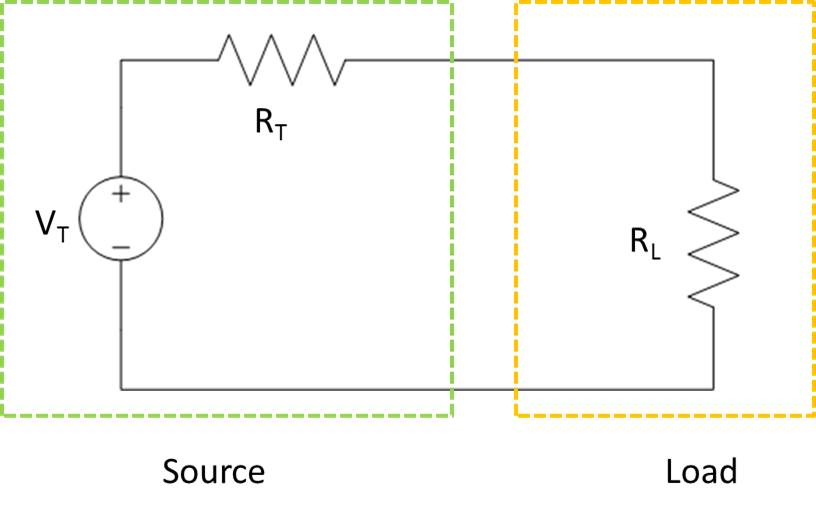
\includegraphics[width=0.5\textwidth]{Source_Load.jpg}
\caption{Circuit showing linear source and load}
\label{fig: Source_Load}
\end{figure}

\textbf{What do we mean by maximum power transfer?}

\soln{1in}{
This is the condition when the power consumed by the load is at its maximum.
}

\newpage
\pagebreak
\clearpage

\textbf{What are the conditions for maximum power transfer?}

Assume in this discussion that we cannot control $R_T$.  This entire discussion will reference Figure \ref{fig: Source_Load}

Start by writing an equation for the voltage across the load resistor:
\soln{1in}{
\begin{equation}
	V_T = i_{load}(R_L + R_T) \\
	i_{Load}=\frac{R_L}{R_L+R_T}V_T
\end{equation}

You should be able to easily recognize that $v_{Load}$ gets larger as $R_L$ gets larger; if $R_L=\infty$ then $v_{Load}=V_T$ which is the max value it can take on.
}

Next, let's find the current in the loop:
\soln{1in}{
\begin{equation}
i_{Load}=\frac{V_T}{R_L + R_T}
\end{equation}

It should be easy to see that $i_{Load}$ grows as $R_L$ get smaller. If $R_L=0$ this $i_{Load}=i_{sc}=\frac{V_T}{R_T}$
}

But
\begin{equation}
P_{Load}=v_{Load}i_{Load}
\end{equation}

which, using previous equations, is:

\soln{1in}{
\begin{equation}
P_{Load}=\frac{R_L}{R_L+R_T}V_T\frac{V_T}{R_L + R_T}
\end{equation}
\begin{equation}
P_{Load}=\frac{R_LV_T^2}{(R_L+R_T)^2}
\end{equation}
}

\textbf{How can we maximize this equation?}

\soln{5in}{
Take the derivative (with respect to $R_L$) and set it equal to zero!

To take this derivative we need to use the quotient rule:

If
\begin{equation}
f(x) = \frac{g(x)}{h(x)}
\end{equation}
then
\begin{equation}
\frac{\partial{f(x)}}{\partial{x}}=\frac{h(x)\partial{g(x) -g(x)\partial{h(x)}}}{h^2(x)}
\end{equation}

So,

\begin{equation}
\frac{\partial{P}}{\partial{R_L}}=\frac{(R_L+R_T)^2V_T^2-2R_LV_T^2(R_L+R_T)}{(R_L + R_T)^4}
\end{equation}
which will simplify to
\begin{equation}
\frac{\partial{P}}{\partial{R_L}}=V_T^2\frac{R_T - R_L}{(R_L + R_T)^3}
\end{equation}

If we set that equal to zero
\begin{equation}
V_T^2\frac{R_T - R_L}{(R_L + R_T)^3}=0
\end{equation}

Then solve for $R_L$
\begin{equation}
R_L=R_T
\end{equation}

}

\textbf{Now find the value for $R_T$ that gives max power, what is the maximum power delivered?}
\soln{2in}{
Plug $R_L=R_T$ into the power equation and solve to get
\begin{eqnarray}
P_{Load}=\frac{R_TV_T^2}{(2R_L)^2}= \frac{R_TV_T^2}{4R_T^2}=\frac{V_T^2}{4R_T}=P_{MAX} \\
P_{MAX}=\frac{V_T^2}{4R_T}=\frac{V_T i_N}{4}=\frac{i_N^2 R_T}{4}
\end{eqnarray}
}

Note, $P_{MAX}$ does not imply maximum efficiency too (see book p. 120 for more details).

\section{Examples}
\subsection{Example 1 - Textbook Exercise 3-33}
A source circuit delivers $4\ V$ to a $50\Omega$ load and $5\ V$ to a $75\Omega$ load.  Find the maximum voltage, current, and power available from the source.
\soln{6in}{
\begin{figure} [h t b]
\centering
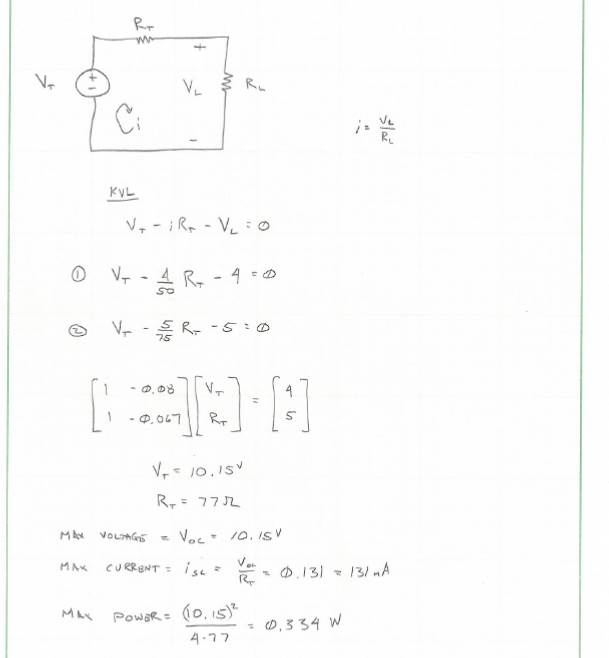
\includegraphics[width=0.9\textwidth]{Example1soln.jpg}
\end{figure}
}

\newpage
\pagebreak
\clearpage

\subsection{Example 2}
For the circuit shown in Figure \ref{fig: Example2}, find the value of $R_L$ that gives maximum power transfer and find the maximum amount of power absorbed by $R_L$.
\begin{figure} [h t b]
\centering
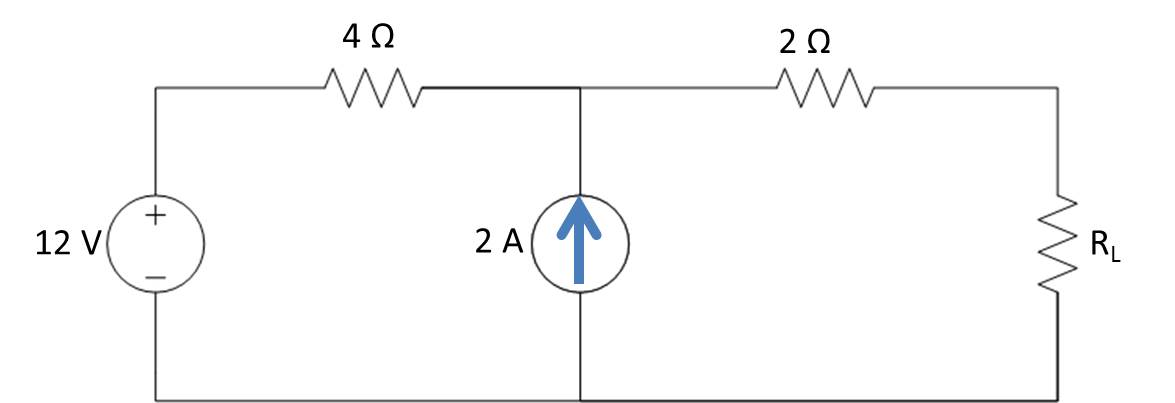
\includegraphics[width=0.6\textwidth]{Example2.jpg}
\caption{Example 2 Circuit}
\label{fig: Example2}
\end{figure}

\soln{6in}{
\begin{figure} [h t b]
\centering
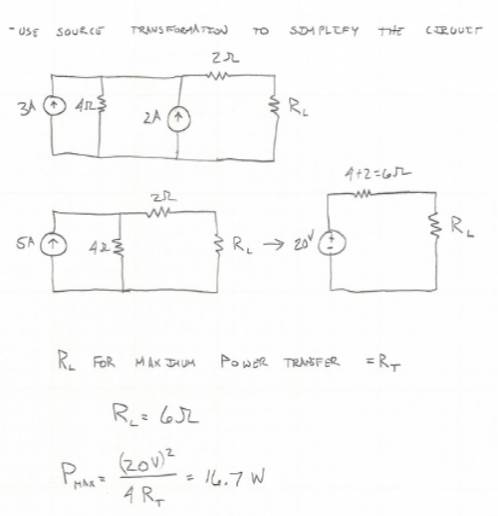
\includegraphics[width=0.9\textwidth]{Example2soln.jpg}
\end{figure}
}

\newpage
\pagebreak
\clearpage

\subsection{Example 3}
For the circuit shown in Figure \ref{fig: Example3}, find the value of $R_L$ that gives maximum power transfer and find the maximum amount of power absorbed by $R_L$.
\begin{figure} [h t b]
\centering
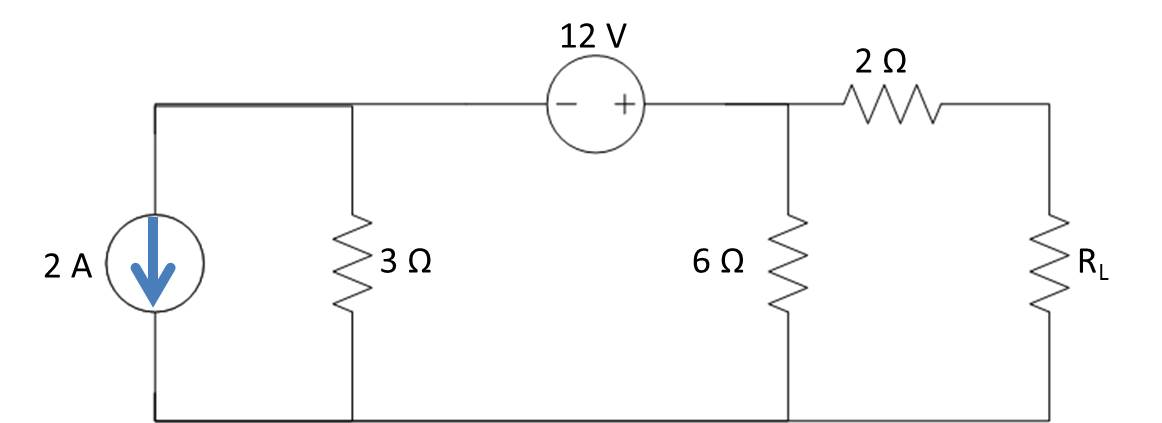
\includegraphics[width=0.5\textwidth]{Example3.jpg}
\caption{Example 3 Circuit}
\label{fig: Example3}
\end{figure}

\soln{6in}{
\begin{figure} [h t b]
\centering
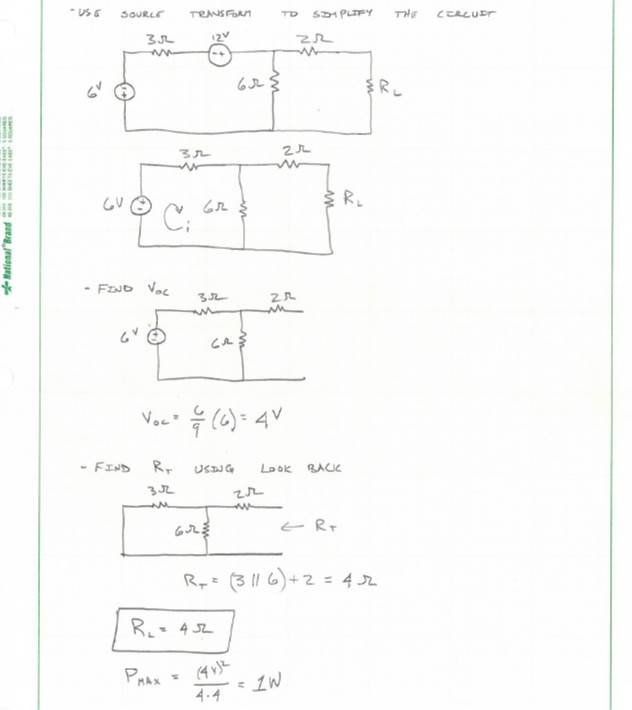
\includegraphics[width=0.7\textwidth]{Example3soln.jpg}
\end{figure}
}

\newpage
\pagebreak
\clearpage

\end{document}


% Equation Array Example Code
%\begin
%{eqnarray}
%P_R &=& i_R^2R \nonumber \\
%P_R &=& (100\ mA)^2 \times 100\ \Omega \nonumber \\
%P_R &=& (100 \times 10^{-3}\ A)^2 \times 100\ \Omega \\
%P_R &=& 10000 \times 10^{-6}\ A^2  \times 100\ \Omega \nonumber \\
%P_R &=& 1\ W  \nonumber
%\end{eqnarray}

% Figure Example Code
%\begin{figure} [h t b]
%\centering
%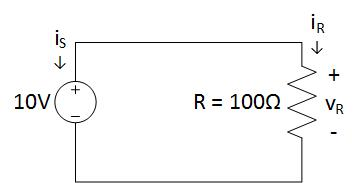
\includegraphics[width=0.5\textwidth]{OhmsLawExampleSolution.jpg}
%\caption{Ohm's Law example circuit}
%\label{fig: OhmsLawExampleSolution}
%\end{figure}

%Table Example Code
%\begin{table}[h]
%\centering
%\begin{tabular}{|l|c|c|}
%\hline
%Prefix & Abbreviation & Value \\
%\hline \hline
%Giga & $G$ & $10^9$ \\
%Mega & $M$ & $10^6$ \\
%Kilo & $k$ & $10^3$ \\
%\hline
%milli & $m$ & $10^{-3}$ \\
%micro & $\mu$ & $10^{-6}$ \\
%nano & $n$ & $10^{-9}$ \\
%pico & $p$ & $10^{-12}$ \\
%\hline
%\end{tabular}
%\caption{Engineering prefixes and values}
%\label{tab: Eng Prefixes}
%\end{table}
